% =========================================================================
\section{Hidden Brokers and What Selects Them (RQ2)}
\label{sec:brokers}

\subsection{Scoring structural position}
\label{sec:instrument}
The criterion needs a score $s$ of structural centrality that works on a
ledger where most addresses carry no label. We obtain it by predicting the
\emph{core} label of Section~\ref{sec:data} from structure alone: a logistic
regression (standardised inputs, balanced class weights) evaluated by
stratified five-fold cross-validation with shuffling. The label never enters
the inputs. Table~\ref{tab:instrument} compares four inputs, and a constant-input control, on the $10^{4}$
subgraphs: PageRank and sampled betweenness alone; the seven hand-crafted
structural features of Section~\ref{sec:data}; and two learned
16-dimensional embeddings, an unsupervised two-layer GraphSAGE encoder
\cite{hamilton2017inductive} (hidden width 32, 200 epochs, Adam with learning
rate 0.01, link-reconstruction objective with negative sampling) and
node2vec. Learned embeddings are averaged over independent initialisations.

\begin{table}[t]
\centering\small
\caption{Cross-validated AUC for predicting the core label from structure
($10^{4}$ subgraphs). Fold avg.: mean of the five fold AUCs (GNN: mean
$\pm$ s.d.\ over ten initialisations; node2vec: five). Pooled: one AUC over
all out-of-fold predictions, the basis of the bootstrap intervals in the
text; for GraphSAGE the median over the ten single-seed models, and a
separate row for the ten-seed ensemble. Differences quoted in the text are
computed before rounding. Anchors: number of core-labelled nodes.}
\label{tab:instrument}
\setlength{\tabcolsep}{3pt}\footnotesize
\begin{tabular}{@{}lcccc@{}}
\toprule
& \multicolumn{2}{c}{LINK} & \multicolumn{2}{c}{UNI} \\
\cmidrule(lr){2-3}\cmidrule(l){4-5}
Input & Fold avg. & Pooled & Fold avg. & Pooled \\
\midrule
PageRank + betw. & \V{c1.link.cent} & \V{aci.link.pool.cent} & \V{c1.uni.cent} & \V{aci.uni.pool.cent} \\
Structural features (7) & \V{c1.link.struct} & \V{aci.link.pool.struct} & \V{c1.uni.struct} & \V{aci.uni.pool.struct} \\
GraphSAGE, single seed & \V{c1.link.gnn} & \V{aci.link.pool.gnn_single} & \V{c1.uni.gnn} & \V{aci.uni.pool.gnn_single} \\
GraphSAGE ensemble & --- & \V{aci.link.pool.gnn_ens} & --- & \V{aci.uni.pool.gnn_ens} \\
node2vec & \V{c1.link.n2v} & --- & \V{c1.uni.n2v} & --- \\
GraphSAGE, const.\ input & \V{c1.link.nofeat} & --- & \V{c1.uni.nofeat} & --- \\
\midrule
Nodes / anchors & \multicolumn{2}{c}{\V{link.nodes.1w} / \V{link.anchors.1w}} & \multicolumn{2}{c}{\V{uni.nodes.1w} / \V{uni.anchors.1w}} \\
\bottomrule
\end{tabular}
\end{table}

The gap that matters is between the two-feature centrality baseline and
everything else. The seven structural features, which include degree and
counterparty count, recover the label nearly as well as either learned
embedding; the GraphSAGE embedding exceeds them by \V{c1.link.gnn_margin} on
LINK and \V{c1.uni.gnn_margin} on UNI in fold-averaged AUC. With only
\V{link.anchors.1w} and \V{uni.anchors.1w} positives, seed-level standard
deviations understate the uncertainty, so we also bootstrap nodes over pooled
out-of-fold predictions (Table~\ref{tab:instrument}, pooled columns). The
structural features beat centrality by \V{aci.link.struct_cent} (95\% CI
\V{aci.link.struct_cent.ci}) on LINK and \V{aci.uni.struct_cent}
(\V{aci.uni.struct_cent.ci}) on UNI. The ten-seed GraphSAGE ensemble beats
the structural features by \V{aci.link.gnn_struct}
(\V{aci.link.gnn_struct.ci}) and \V{aci.uni.gnn_struct}
(\V{aci.uni.gnn_struct.ci}), only just distinguishable from zero. Part of
that margin is the ensemble rather than the representation: the structural
features are a single model, and a single GraphSAGE model beats them by a
median \V{aci.link.single.diff} on LINK (\V{aci.link.single.range} across
seeds) and \V{aci.uni.single.diff} on UNI (\V{aci.uni.single.range}), with
the 95\% interval excluding zero for \V{aci.link.single.nexcl} and
\V{aci.uni.single.nexcl} of the ten seeds respectively. What separates good from poor
inputs is therefore mainly whether they contain degree and counterparty
information, not whether they are learned.
Replacing all inputs with a constant collapses the GraphSAGE embedding to
chance, a degeneracy of mean aggregation over uninformative inputs; node2vec,
which uses topology alone, shows that topology is informative. On the
$5\times10^{4}$ and full LINK graphs the ordering is the same
(\ref{app:instrument}). We use the GraphSAGE score as $s$ and treat that
choice as a parameter.

\subsection{The criterion}
\label{sec:criterion}
A node is a hidden broker if (i) its score $s$ is in the top 1\%, (ii) its
balance is at most the median balance of the subgraph, (iii) it has
at least five distinct counterparties, (iv) its sampled betweenness is
positive, and (v) it is unlabelled in the archived compilation. Conditions
(iii) and (iv) exclude addresses that cannot sit on any path. Because a hard
percentile cut is sensitive to initialisation, $s$ is the mean percentile
rank over ten independently initialised embeddings, cut once.
The median in condition (ii) is zero on UNI, where \V{uni.zero_share} of the
subgraph's nodes hold nothing, and \V{link.med_bal} LINK on LINK, where
\V{link.zero_share} hold nothing and the median node holds a residue of order
$10^{-5}$ tokens. Condition (ii) therefore admits zero or
dust balances: \V{link.brokers_zero_bal} of the LINK brokers and
\V{uni.brokers_zero_bal} of the UNI brokers hold exactly zero
(Table~\ref{tab:brokerspec} gives the sets under a strict zero-balance
condition and under a 0.01-token dust floor).

Under the main specification the criterion selects \V{link.brokers} addresses
on LINK and \V{uni.brokers} on UNI, \V{shared.brokers} of them on both. An
alternative rule---selection in at least half of the ten individual runs---gives
\V{link.brokers_vote} and \V{uni.brokers_vote}, and the two rules agree on
\V{link.brokers_both} and \V{uni.brokers_both}. A betweenness-based selection
of the same size from the same pool shares \V{link.brokers_bet_overlap} and
\V{uni.brokers_bet_overlap} addresses with the GraphSAGE selection.

\subsection{What the selected set depends on}
\label{sec:stability}
\paragraph{Initialisation}
Training is deterministic for a given seed (\ref{app:repro}); across the ten
seeds, \V{link.brokers_ever} LINK addresses are selected at least once and
\V{link.brokers_rare} of them at most twice, which is why we report the rank
ensemble rather than a single run.

\paragraph{Data cleaning}
The selected set moves with the cleaning specification
(Table~\ref{tab:brokerspec}). Of the \V{v1.link.brokers} LINK and
\V{v1.uni.brokers} UNI brokers reported in the first version of this paper,
which used uncleaned transfers, \V{link.brokers_v1_kept} and
\V{uni.brokers_v1_kept} remain, and the number shared by the two ledgers
falls from \V{v1.shared.brokers} to \V{shared.brokers}. The causes differ by
ledger. On LINK the change is mainly the cleaning: with both cleaning rules
switched off, the present pipeline recovers \V{link.brokers_v1_raw} of the
first version's \V{v1.link.brokers}. On UNI, where cleaning removes almost
nothing and every cleaning specification gives the same set
(Table~\ref{tab:brokerspec}), the change comes from the end-of-window balance
snapshot and from the determinism corrections of \ref{app:repro}: only
\V{uni.brokers_v1_raw} of the first version's \V{v1.uni.brokers} are
recovered even without cleaning. With the airdrop transfers kept, the LINK set
has \V{spec.link.brokers.keep_airdrop} members, of which
\V{spec.link.overlap.keep_airdrop} are in the main set; with zero-value
transfers kept it has \V{spec.link.brokers.keep_zero}
(\V{spec.link.overlap.keep_zero} shared). On UNI, where the airdrop rule
removes nothing, keeping zero-value transfers alone gives a set of
\V{spec.uni.brokers.keep_zero}, of which \V{spec.uni.overlap.keep_zero} are in the main set.

\begin{table}[t]
\centering\small
\caption{Hidden-broker sets under the cleaning specifications of
\ref{app:cleaning} and under two alternative balance conditions (ii): size,
and overlap with the main set. Balance-condition rows reuse the main
ensemble scores; the addresses they add to the main set (\V{bsens.link.dust.new} on
LINK and \V{bsens.uni.dust.new} on UNI under the dust condition) were not verified.}
\label{tab:brokerspec}
\begin{tabular}{@{}lcccc@{}}
\toprule
& \multicolumn{2}{c}{LINK} & \multicolumn{2}{c}{UNI} \\
\cmidrule(lr){2-3}\cmidrule(l){4-5}
Specification & Size & Overlap & Size & Overlap \\
\midrule
\textbf{Main} & \V{link.brokers} & --- & \V{uni.brokers} & --- \\
Zero-value kept & \V{spec.link.brokers.keep_zero} & \V{spec.link.overlap.keep_zero} & \V{spec.uni.brokers.keep_zero} & \V{spec.uni.overlap.keep_zero} \\
Airdrop kept & \V{spec.link.brokers.keep_airdrop} & \V{spec.link.overlap.keep_airdrop} & \V{spec.uni.brokers.keep_airdrop} & \V{spec.uni.overlap.keep_airdrop} \\
Both kept & \V{spec.link.brokers.raw} & \V{spec.link.overlap.raw} & \V{spec.uni.brokers.raw} & \V{spec.uni.overlap.raw} \\
Edges overwritten & \V{spec.link.brokers.overwrite} & \V{spec.link.overlap.overwrite} & \V{spec.uni.brokers.overwrite} & \V{spec.uni.overlap.overwrite} \\
\addlinespace[2pt]
\multicolumn{5}{@{}l}{\emph{Balance condition (main data)}} \\
Balance exactly zero & \V{bsens.link.zero.size} & \V{bsens.link.zero.overlap} & \V{bsens.uni.zero.size} & \V{bsens.uni.zero.overlap} \\
Balance $<$ 0.01 tokens & \V{bsens.link.dust.size} & \V{bsens.link.dust.overlap} & \V{bsens.uni.dust.size} & \V{bsens.uni.dust.overlap} \\
\bottomrule
\end{tabular}
\end{table}

\paragraph{Representation}
node2vec, scored and cut in the same way, selects \V{link.n2v_brokers} LINK
addresses, of which \V{link.n2v_overlap} are also in the GraphSAGE set. Among
its top percentile \V{link.n2v_top1_labelled} of nodes carry a label, against
\V{link.gnn_top1_labelled} for GraphSAGE: node2vec ranks catalogued
infrastructure highest, and that infrastructure is removed by condition (v).

\subsection{Does the representation add anything? A matched control}
\label{sec:control}
That the selected addresses turn out to be routing infrastructure does not by
itself show the selection was informative, since we inspected only what it
chose. We therefore drew controls from the same eligibility pool---conditions
(ii)--(v) without (i)---restricted to addresses not selected, and verified
them blind. The pool's median counterparty count is \V{ctl.pool_med_cp}
against \V{ctl.broker_med_cp} for the brokers, so an unmatched control would
differ in degree as well as in selection; the main control matches each of 20
brokers, drawn at random, to the unselected address closest in counterparty
count. Group sizes (20 matched, 10 unmatched, 8 broker anchors) and the random
seed were fixed in advance, sized to detect a difference of 30 percentage
points (35\% against 5\%) with a one-sided Fisher test; at the observed
matched-control rate, 80\% power at $\alpha = 0.05$ requires a difference of
about \V{ctl.mdd} points. Controls, anchors and
any broker without an earlier verification record were shuffled into one list
without group labels and verified by one author; addresses verified in the
first version of this paper keep that record. Verification uses Etherscan
name tags, verified source and deployer, and the token-transfer history, and
assigns one of: a named protocol, an unlabelled routing contract, an MEV bot,
or unknown. Centralized-exchange deposit and hot-wallet addresses are not
routing protocols and are scored as unknown; we fixed this rule before
unblinding, and it changes only the unmatched group
(\ref{app:control}).

The blinded anchors were judged exactly as in the earlier record
(\V{ctl.anchor_agree} anchors), and resolve to named protocols at
\V{ctl.anchor_pct} against \V{ctl.broker_pct} for all brokers, so the standard
did not shift under blinding. Of the 20 matched controls, \V{ctl.matched_k}
(\V{ctl.matched_pct}, 95\% CI \V{ctl.matched_ci}) resolve to a named protocol,
against \V{ctl.broker_k} of \V{link.brokers} brokers (\V{ctl.broker_pct},
\V{ctl.broker_ci}); one-sided Fisher exact $p = \V{ctl.p}$. Of the ten
unmatched controls, \V{ctl.uniform_k} do (\V{ctl.uniform_pct},
\V{ctl.uniform_ci}); the difference between matched and unmatched controls is
in the expected direction but not significant ($p = \V{ctl.p_mu}$).

\begin{figure}[t]
  \centering
  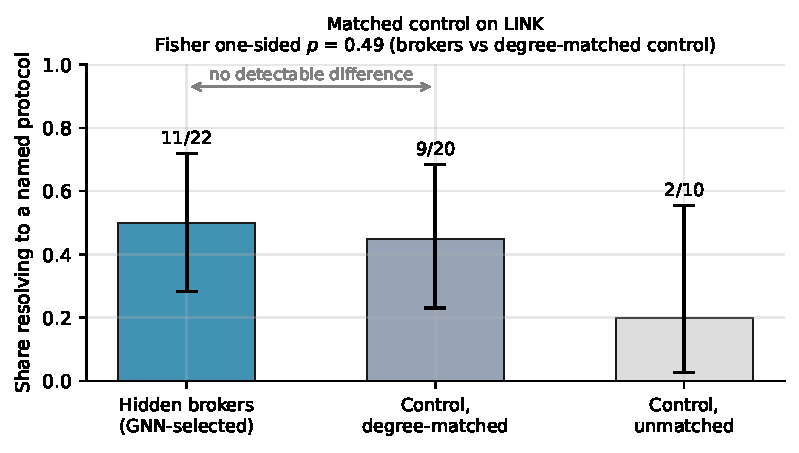
\includegraphics[width=\linewidth]{fig_random_control.pdf}
  \caption{Matched control on LINK: share of each group resolving to a named
  routing protocol under blind verification, with Clopper--Pearson 95\%
  intervals. Matched controls come from the same eligibility pool as the
  brokers and are matched on counterparty count.}
  \label{fig:control}
\end{figure}

Conditional on counterparty count, then, the learned score adds nothing we
can detect (Fig.~\ref{fig:control}). The 95\% interval for the difference between brokers and matched
controls is \V{ctl.diff_ci} percentage points: it excludes an advantage of
more than about a third, but not a small one, so the defensible statement is
that no advantage was detected. Either way, the finding that these addresses are
routing infrastructure does not depend on the representation used to surface
them.

\subsection{Verification and live labels}
\label{sec:verify}
Every address in the union of the two broker sets (\V{brokers.union}
addresses) has a manual verification record, and \V{brokers.union_named}
resolve to a named protocol: DEX aggregators and swap routers, intent
solvers, wallet swap interfaces and cross-chain routers. ``Unlabelled'' is
relative to the archived compilation, not to the block explorer: checked on
6 October 2026, \V{brokers.live_tagged} of the \V{brokers.union} carry an
Etherscan public name tag and \V{brokers.live_untagged} do not. The
compilation's gaps are largely a matter of age. Of the \V{deploy.n_contracts}
contracts among the brokers (the remaining address is an exchange wallet),
\V{deploy.n_after} were deployed after the compilation was last scraped in
June 2023; the other two, MetaMask's swap spender (2020) and LI.FI's router
(2022), predate it and are missing anyway. A hidden broker is therefore, for
the most part, routing infrastructure newer than the label set used to look
for it, and the criterion is best read as a way of finding what a dated label
set misses. Of the \V{shared.brokers} addresses selected on both
ledgers, \V{shared.brokers_named} are named protocols
(\V{shared.brokers_names}); the remaining one is an unlabelled routing
contract. Structural coreness is agnostic to legitimacy:
the union also contains MEV bots and a centralized-exchange hot wallet absent
from the compilation, so the signature---many counterparties, no
custody---identifies operational centrality, not role or intent.
